\documentclass[12pt]{ociamthesis}  % default square logo 
%\documentclass[12pt,beltcrest]{ociamthesis} % use old belt crest logo
%\documentclass[12pt,shieldcrest]{ociamthesis} % use older shield crest logo

%load any additional packages
\usepackage{amssymb}
\usepackage[T1]{fontenc}
\usepackage[polish]{babel}
\usepackage{hyperref}
\usepackage[table]{xcolor}
\usepackage{float}
\usepackage[utf8]{inputenc}
\usepackage{graphicx}
\graphicspath{ {./images/theory/}{./images/RoR/}{./images/spring/} }
%input macros (i.e. write your own macros file called mymacros.tex 
%and uncomment the next line)
%\include{mymacros}

\title{Tworzenie REST API w oparciu o frameworki Ruby on Rails i Spring}      %your thesis title,
 
\author{Mateusz Czajka}             %your name
\college{Wydział Matematyki i Informatyki}  %your college

%\renewcommand{\submittedtext}{change the default text here if needed}
\degree{Praca inżynierska}     %the degree
\degreedate{Poznań 2022}         %the degree date

%end the preamble and start the document
\begin{document}

%this baselineskip gives sufficient line spacing for an examiner to easily
%markup the thesis with comments
\baselineskip=18pt plus1pt

%set the number of sectioning levels that get number and appear in the contents
\setcounter{secnumdepth}{3}
\setcounter{tocdepth}{3}

%set settings for tables
\setlength{\tabcolsep}{8pt}
\renewcommand{\arraystretch}{2}


\maketitle                  % create a title page from the preamble info

%\begin{romanpages}          % start roman page numbering
\tableofcontents            % generate and include a table of contents
%\listoffigures              % generate and include a list of figures
%\end{romanpages}            % end roman page numbering
\chapter*{Wstęp}
	Praca ma na celu przedstawienie czym jest, oraz jak tworzyć REST API z wykorzystaniem protokołu HTTP. Na początku omówione zostaną podstawowe pojęcia związane z REST API. Praca przedstawi protokół HTTP, w kontekście używania go w architekturze REST, wraz z jego własnościami, metodami oraz kodami odpowiedzi. Następnie przedstawiona zostanie sama architektura REST oraz zasady według których powinna być implementowana. W kolejnym rozdziale praca skupi się przede wszystkim na praktycznych aspektach tworzenia REST API. Omówione zostaną dobre praktyki, których warto się trzymać podczas programowania interfejsu sieciowego. W tej sekcji pokazane zostaną również częste problemy, które można napotkać podczas tworzenia REST API oraz sposoby na ich rozwiązanie. Dodatkowo praca opisze pewne aspekty związane z bezpieczeństwem podczas projektowania interfejsów sieciowych. Na sam koniec przedstawiony zostanie plan tworzenia serwisu RESTful. Wszystko to w oparciu o przykłady stworzone przy pomocy dwóch popularnych frameworków: Ruby on Rails oraz Spring.
	
	
	 

%now include the files of latex for each of the chapters etc
\chapter{HTTP, API, REST}
\section{HTTP}
	Protokół HTTP (Hypertext Transfer Protocol) jest fundamentem, na którym postawiona jest współczesna komunikacja w internecie. HTTP działa w architekturze klient-serwer co oznacza, że zapytania, inicjowane przez odbiorcę (najczęściej przeglądarkę internetową), wysyłane są do serwera, a ten zwraca określoną odpowiedź. W celu wyświetlenia strony internetowej przeglądarka wysyła żądanie pobrania dokumentu HTML, który reprezentuje stronę WWW. Następnie przeglądarka analizuje otrzymany plik, wykonuje dodatkowe żądania w celu uzyskania informacji na temat układu strony (CSS) i pobrania podzasobów zawartych na stronie (obrazki, filmy video). Przeglądarka łączy wszystkie otrzymane w ten sposób zasoby, aby zaprezentować kompletny dokument - stronę WWW. Skrypty wykonywane przez przeglądarkę mogą pobierać kolejne zasoby w późniejszych fazach, a ta na bieżąco aktualizuje stronę \cite{MozillaHTTP}.

	\subsection{Własności HTTP}
		\begin{enumerate}
			\item niezależny od typów danych - każdy typ danych może być przesyłany za pomocą HTTP, o ile zarówno klient, jak i serwer wiedzą, jak je obsłużyć. Wymagane jest, aby zarówno klient, jak i serwer określili typ zawartości za pomocą odpowiedniego typu MIME (Multipurpose Internet Mail Extensions - standard, który wskazuje, jaki rodzaj dokumentu, pliku lub strumienia bajtów jest przesyłany).
			
			\item rozszerzalny - nagłówki HTTP pozwalają w łatwy sposób dodać nowe parametry do protokołu. Należy jedynie ustalić semantykę nowego nagłówka między klientem a serwerem. Niestandardowe nagłówki wykorzystuje się w celu przesyłania dodatkowych danych na temat żądań i odpowiedzi.
			
			\item bezstanowy, ale nie bez sesji - serwer i klient są świadomi siebie nawzajem tylko podczas bieżącego żądania. Oznacza to, że nie ma powiązania między dwoma żądaniami wykonywanymi kolejno przez tego samego klienta. Dla użytkowników, którzy chcą w ciągły sposób wchodzić w interakcję z niektórymi stronami (np. poruszać się jako zalogowany użytkownik po aplikacji e-learningowej), może stanowić do duży problem. Jednym z rozwiązań tego problemu są ciasteczka HTTP. Te pozwalają na stworzenie sesji dla każdego zapytania w celu udostępnienie tego samego kontekstu lub stanu.
			
			\item niezawodny - protokół powinien być niezawodny, przesyłane wiadomości nie mogą być tracone. Wśród dwóch najpopularniejszych protokołów służących do transportowania danych w internecie (TCP/UDP) TCP jest niezawodny. Oznacza to, że sam protokół posiada mechanizmy sprawdzające, czy wszystko, co zostało przesłane, dotarło do odbiorcy i właśnie z tego powodu HTTP oparty jest na standardzie TCP.
		\end{enumerate}
	
	\subsection{HTTPS}
		Połączenia z wykorzystaniem protokołu HTTP nie są szyfrowane. Oznacza to, że dane wysyłane przez klienta nie są chronione, w szczególności poufne dane, takie jak hasła. Strony, które opierają swoją komunikację o HTTP, nie są bezpieczne dla użytkowników i odchodzi się od nich na rzecz HTTPS.
		
		HTTPS (Hypertext Transfer Protocol Secure) to rozszerzenie HTTP, które wykorzystywane jest do bezpiecznej komunikacji w internecie. Protokół komunikacji jest szyfrowany przy pomocy Transport Layer Security (TLS) lub wcześniej Secure Sockets Layer (SSL) \cite{WikipediaHTTPS}.
		
		HTTPS tworzy bezpieczny kanał, który chroni przed atakami podsłuchującymi i atakami typu "man-in-the-middle", pod warunkiem, że stosowane są odpowiednie pakiety szyfrowania, a certyfikat serwera jest zaufany i zweryfikowany.
	
	\subsection{Metody HTTP}
		HTTP definiuje dziewięć metod, które pozwalają określić jaka akcja powinna zostać wykonana dla określonego zasobu \cite{MozillaHTTPMethods}.
		
		\begin{itemize}
			\item GET - żąda reprezentacji określonego zasobu. Żądania używające metody GET powinny być wykorzystywane jedynie do pobierania danych \cite{RESTfulWebServices}.
			\item HEAD - żąda takiej samej odpowiedzi jak GET, ale bez treści odpowiedzi (response body).
			\item POST - wysyła dane do serwera, najczęściej w celu stworzenia zasobu.
			\item PUT - wysyła dane do serwera w celu zastąpienia zasobu nową reprezentacją.
			\item PATCH - wysyła dane do serwera w celu częściowej aktualizacji zasobu.
			\item DELETE - usuwa określony zasób.
			\item CONNECT - ustanawia tunel do serwera.
			\item OPTIONS - opisuje możliwości komunikacji.
			\item TRACE - wykonuje test zwrotny do zasobu docelowego.
		\end{itemize}
		
	\subsection{Kody odpowiedzi HTTP}
		Kod odpowiedzi HTTP informuje użytkownika o statusie żądania HTTP. Kody są podzielone na pięć grup: \cite{MozillaHTTPStatuses}
		\begin{enumerate}
			\item kody informacyjne (100 - 199)
			\item kody powodzenia (200 - 299)
			\item kody przekierowania (300 - 399)
			\item kody błędu aplikacji klienta (400 - 499)
			\item kody błędu aplikacji serwera (500 - 599)
		\end{enumerate}
		Powyższe kody odpowiedzi są zdefiniowane przez \href{https://httpwg.org/specs/rfc9110.html#overview.of.status.codes}{RFC 9110}. Popularne kody odpowiedzi:
		\begin{itemize}
			\item 200 OK - zapytanie się powiodło.
			\item 201 Created - zapytanie powiodło się i powstał nowy zasób.
			\item 204 No Content - zapytanie powiodło się, ale nie ma dla niego treści odpowiedzi.
			\item 301 Moved Permanently - URL zasobu zmieniło się na stałe. Nowe URL jest podawane w odpowiedzi.
			\item 302 Found - zasób został odnaleziony, jednak nie w miejscu, w którym go oczekiwano.
			\item 400 Bad Request - serwer nie obsłuży zapytanie z powodu błędu w zapytaniu klienta.
			\item 401 Unauthorized - klient musi się uwierzytelnić, aby otrzymać odpowiedź od serwera.
			\item 403 Forbidden - klient nie ma uprawnień do zawartości.
			\item 404 Not Found - serwer nie może znaleźć żądanego zasobu. Oznacza to, że URL nie jest rozpoznane lub zasób nie istnieje.
			\item 405 Method Not Allowed - użyta została nieodpowiednia metoda HTTP.
			\item 415 Unsupported Media Type - rodzaj danych wysłanych w zapytaniu nie jest obsługiwany przez serwer.
			\item 500 Internal Server Error - serwer napotkał na sytuację, z którą nie jest w stanie sobie poradzić.
			\item 502 Bad Gateway - serwer otrzymał nieprawidłową odpowiedź, kiedy próbował uzyskać odpowiedź potrzebną do obsłużenia zapytania.
			\item 503 Service Unavailable - serwer nie jest gotowy do obsłużenia zapytania.
		\end{itemize}

\section{API}
	API (Application Programming Interface) jest specyfikacją wytycznych opisujących, w jaki sposób programy komunikują się między sobą. Oprogramowanie upublicznia interfejs dla świata zewnętrznego (użytkowników sieci lub innych programów i serwisów). API jest tworzone, aby programy mogły komunikować się ze sobą, lecz muszą być zrozumiałe dla człowieka, który jest odpowiedzialny za kod aplikacji \cite{DesigningWebAPIs}.
	
	Interfejsy API są kluczowym komponentem, który umożliwia funkcjonowanie aplikacjom w internecie. API pozwala na zamówienie pizzy przez internet, zapłatę za subskrypcję VOD, obejrzenie filmu video i wiele więcej.
	

\section{Architektura REST}
	Przed rokiem 2000 nie istniał standard, który mówił, w jaki sposób tworzyć i używać API w sieci Internet. Integracje wymagały użycia protokołów takich jak SOAP, które były trudne do implementacji, utrzymania i debugowania. Dopiero Roy Fielding w swojej pracy "Architectural Styles and the Design of Network-based Software Architectures" \cite{ArchitecturalStyles} stworzył REST (Representational state transfer), który ustandaryzował tworzenie i korzystanie z API. Celem pracy było stworzenie standardu, który pozwoli dwóm serwerom na komunikacje i wymianę informacji z dowolnego miejsca na świecie. Z tego powodu zaprojektowano szereg zasad, właściwości i ograniczeń, które nazwano REST. REST to architektura oparta na zasobach, jednolitości interfejsu, architekturze klient-serwer, bezstanowości, używająca cachu i wykorzystująca protokół do przesyłania danych (najczęściej HTTP).
	
	\subsection{REST API}
		REST to obecnie najpopularniejsza architektura wybierana przez programistów do tworzenia API \cite{DesigningWebAPIs}. API tworzone na podstawie paradygmatów REST nazywane jest REST API (lub RESTful API).
		
		Zapytanie wysyłane za pomocą interfejsu REST API przekazuje reprezentację stanu zasobu do odpowiedniego endpointu aplikacji. Dane są dostarczane przy pomocy HTTP w określonym formacie (zazwyczaj JSON/XML). Najczęściej używanym typem danych jest jednak JSON, ponieważ jest niezależny od języka, czytelny dla człowieka oraz prosty do parsowania. Ważnym elementem zapytań REST API są nagłówki i parametry HTTP. Mogą one zawierać ważne informacje identyfikacyjne, takie jak metadane żądania, uprawnienia, URI (Uniform Resource Identifier - sekwencja znaków, która identyfikuje zasób np. example.com/api/v1/companies/:companyID \cite{RESTAPIDesignRulebook}), ciasteczka i inne.
	
	
	\subsection{Zasady REST API}
		Kilka podstawowych zasad, które należy przestrzegać w trakcie tworzenia REST API z wykorzystaniem HTTP:
		\begin{itemize}
			\item Kody odpowiedzi HTTP są zwracane przez serwer w celu poinformowania o stanie zapytania. Kody odpowiedzi 2XX informują o sukcesie, 3XX o tym, że zasób został przeniesiony, 4XX o błędzie po stronie klienta, a 5XX o błędzie po stronie serwera \cite{RESTfulWebServices}.
			\item Zasoby są częścią URL (/companies)
			\item Dla każdego zasobu powinny istnieć 2 rodzaje URLi, jeden dla kolekcji (/companies) i drugi dla określonego elementu (/companies/10)
			\item Używa się rzeczowników zamiast czasowników dla akcji związanych z zasobami (zamiast /getCompanyInfo/10 używa się /companies/10)
			\item Metody HTTP (GET, POST, PATCH, PUT, DELETE) informują serwer, jaka akcja powinna zostać wykonana. Różne metody wykonują różne akcje na tym samym URL \cite{RESTfulWebServicesCookbook}.
			\begin{table}[H]
				\begin{tabular}{ |l|l|l|l| } 
					\hline
					%\rowcolor{lightgray}
					Operacja 	& Metoda HTTP 	& /companies 				& /companies/10 		\\ 
					\hline
					Create 		& POST 			& tworzy nową firmę 		& Nie stosuje się 		\\ 
					\hline
					Read 		& GET 			& zwraca wszystkie firmy 	& zwraca firmę 10 		\\ 
					\hline
					Update 		& PATCH/PUT 	& aktualizuje wiele firm 	& aktualizuje firmę 10 	\\ 
					\hline
					Delete 		& DELETE 		& usuwa wszystkie firmy 	& usuwa firmę 10 		\\ 
					\hline	
				\end{tabular}
				\caption{\label{tab:CRUD} CRUD (Create, Read, Update, Delete)}
			\end{table}
			
		
			\item Zasób, który istnieje tylko w innym zasobie (nested resources), powinien być przedstawiony jako zasób podrzędny, a nie jako zasób najwyższego poziomu w adresie URL. Dzięki temu programista korzystający z API klarownie widzi relację między zasobami.
			\begin{table}[H]
				\begin{tabular}{ |l|l|l| } 
					\hline
					%\rowcolor{lightgray}
					Metoda HTTP & /companies/:company/notes 					& /companies/:company/notes/:note 			\\ 
					\hline
					POST 		& tworzy notatkę firmy			& Nie stosuje się 					\\ 
					\hline
					GET 		& zwraca notatki firmy 			& zwraca notatkę firmy 		\\ 
					\hline
					PATCH/PUT 	& aktualizuje notatki firmy 		& aktualizuję notatkę firmy 	\\ 
					\hline
					DELETE 		& usuwa wszystkie notatki firmy 	& usuwa notatkę firmy 			\\ 
					\hline	
				\end{tabular}
				\caption{\label{tab:nested-resources-CRUD} zasób zagnieżdżony - CRUD}
			\end{table}
		
			
			\item Oprócz operacji CRUD, czasami potrzeba zastosować inną operację. W takim wypadku często wykorzystywane są następujące podejścia\cite{DesigningWebAPIs}: 
				\begin{itemize}
					\item Wskazanie na akcje poprzez przekazanie parametru w treści zapytania.
					
					\begin{verbatim}
						PATCH /companies/:company/notes/:note z parametrem {"archived": true}
					\end{verbatim}
					archiwizuję notatkę firmy. \\
				
					\item Traktowanie akcji jak podzasobu.
				
					\begin{verbatim}
						POST /companies/:company/notes/:note/lock
					\end{verbatim}
					blokuję notatkę firmy \\
					
					\item Operacje takie jak szukanie mogą być jeszcze trudniejsze do zaimplementowania w architekturze REST. Typową praktyką w takim przypadku jest użycie czasownika wskazującego na akcje wraz z potrzebnymi parametrami w adresie URL. 
					
					\begin{verbatim}
						GET /companies/:company/notes/search?q="query"
					\end{verbatim}
					wyszukuje odpowiednie notatki  \\
				\end{itemize}
		\end{itemize}
	
		\subsubsection{Spring}
		\begin{figure}[H]
			\begin{center}
				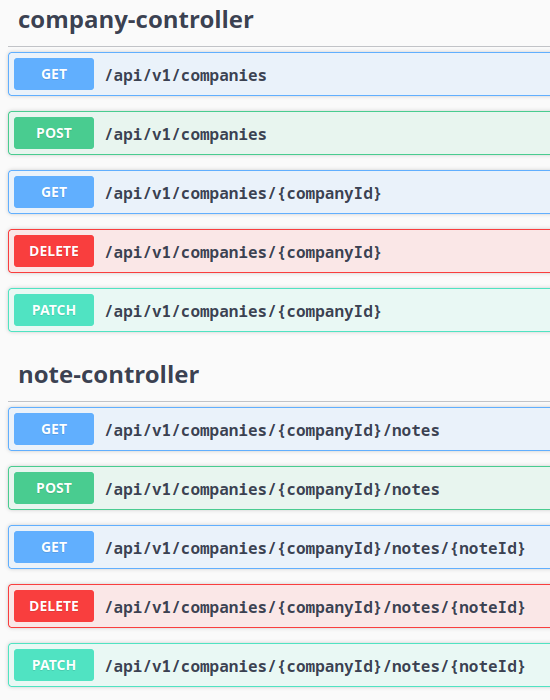
\includegraphics[scale=0.7]{spring_endpoints.png}
				\caption{\label{fig:spring-swagger-endpoints} Spring - endpointy w Swagerze}
			\end{center}
		\end{figure}
		Endpointy do operacji CRUD przygotowane przy pomocy Springa. Company-controller udostępnia standardowe endpointy dla zasobu company. Z kolei note-controller odpowiada za operacje dla zasobu zagnieżdżonego note, który istnieje tylko jako zasób podrzędny względem company.
		
		
		
		\subsubsection{Ruby on Rails}
		Endpointy wygenerowane przy pomocy komendy \cite{RoRDocs}
		\begin{verbatim}
			rails generate scaffold 
		\end{verbatim}
		oraz przygotowaniu zasobu note jako zasobu podrzędnego względem company:
		
		\begin{figure}[H]
			\begin{center}
				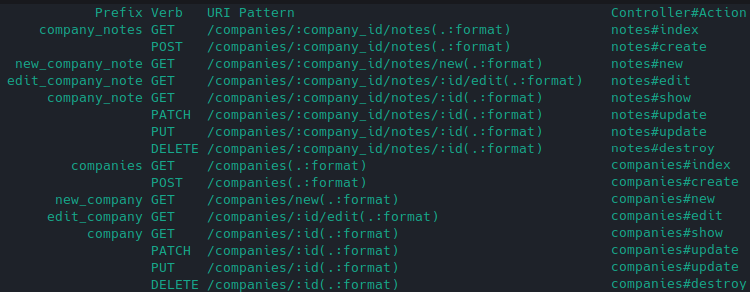
\includegraphics[scale=0.8]{ror_rails_routes.png}
				\caption{\label{fig:ror-endpoints} Ruby on Rails - endpointy}
			\end{center}
		\end{figure}
	
		Jak widać, oprócz podstawowych akcji CRUD Ruby on Rails wygenerował też dwa dodatkowe endpointy, które służą do zwrócenia widoków z formularzami do tworzenia (/companies/new) i akutalizacji (/companies/:id/edit) zasobu company. Warto również zauważyć, że Ruby on Rails dopuszcza metodę PATCH oraz PUT w celu edycji zasobu. Ponadto, do każdego endpointu dodany jest parametr :format, który wskazuje, w jakim formacie danych zostanie zwrócona odpowiedź (obsłużone w kodzie są html oraz json). \\
		
		\noindent Na przykład, dla zapytania:
		\begin{verbatim}
			http://localhost:3000/companies/?format=json
		\end{verbatim}
		zwrócone zostaną dane w formacie json:
		
		\begin{figure}[H]
			\begin{center}
				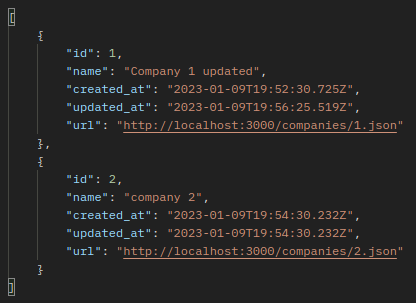
\includegraphics[scale=0.8]{ror_format_json.png}
				\caption{\label{fig:ror-json} Ruby on Rails - odpowiedź json}
			\end{center}
		\end{figure}
	
		
		\noindent Z kolei dla parametru ?format=html zwrócona zostanie zwykła strona html. \\
		
		\noindent Ruby on Rails zwraca również, w odpowiedzi w formacie json, url który po kliknięciu przeniesie użytkownika do konkretnego zasobu.
	
	
	

\chapter{Tworzenie REST API}
\section{Dobre praktyki}
	Interfejsy REST API są obecnie jednym z najbardziej popularnych rodzajów usług w internecie. Pozwalają różnym klientom, w tym przeglądarkom, na komunikację z serwisami sieciowymi. Bardzo ważne jest, aby prawidłowo zaprojektować REST API. Podczas tworzenia API należy wziąć pod uwagę bezpieczeństwo, wydajność oraz łatwość użycia interfejsu dla konsumentów. Z tego powodu warto poznać i stosować się do powszechnie przyjętych konwencji. W przeciwnym razie klienci oraz programiści utrzymujący projekt mogą poczuć się zdezorientowani podczas korzystania z API.
	
	W tej sekcji opisane zostanie kilka praktyk, które warto stosować przy tworzeniu REST API, aby było ono proste w użyciu oraz utrzymaniu.
	
	\subsection{Dokumentacja}
		API jest tak dobre, jak jego dokumentacja. Dokumenty opisujące działanie publicznego API powinny być dostępne publicznie i łatwo wyszukiwalne. Większość programistów sprawdzi dokumentację, zanim podejmie się jakichkolwiek prób integracji, dlatego ukrywanie jej w plikach PDF czy udostępnianie tylko po wcześniejszym zalogowaniu może zniechęcić potencjalnych klientów do korzystania z API.
		
		Dokumentacja powinna zawierać przykłady pełnych żądań i odpowiedzi. Najlepiej, aby przedstawić je w postaci możliwej do łatwego skopiowana (linki, curle lub całe zapytania, których można użyć np. w Postmanie).
		
		Po publicznym udostępnieniu API nie należy wprowadzać do niego żadnych zmian, które sprawią, że programy klientów przestaną poprawnie się z nim komunikować. Dokumentacja musi zawierać informację o poprzednich wersjach API oraz zmianach, które zostały wprowadzone.
		
		\subsubsection{Interaktywna dokumentacja}
		Interaktywna dokumentacja pozwala programistom pracować z API, dając im jasny obraz tego, jak interfejs odpowiada na żądania z różnymi parametrami i opcjami. Zapewnia wszystko, czego deweloperzy potrzebują, aby korzystać z interfejsu przy niewielkim nakładzie czasu i wysiłku. Taka dokumentacja jest niezwykle przydatna, ponieważ umożliwia testowanie, eksperymentowanie i standardowe używanie API. Przykładami narzędzi, które umożliwiają dokumentację oraz korzystanie ze stworzonego API są Postman czy Swagger.
	
	\subsection{Wersjonowanie}
		API powinno mieć określoną wersję. Dzięki temu można wprowadzać zmiany w nowszych wersjach i utrzymywać stare  wersje dla klientów, którzy nie są jeszcze gotowi do migracji ich aplikacji do nowego API. Wersja interfejsu jest najczęściej zawarta w adresie URL, aby zapewnić możliwość przeszukiwania zasobów w przeglądarce oraz ułatwia programistom pracę z API. 
		
		\begin{verbatim}
			http://www.example.com/api/v2/companies, v2 - wersja API
		\end{verbatim}
		
		Bardzo rzadko API będzie całkowicie stabilne. Ważne, aby w odpowiedni sposób informować użytkowników o zachodzących zmianach oraz utrzymywać starsze wersje API. Dobra dokumentacja i odpowiednie wersjonowanie pozwoli zapobiec wielu problemom i sprawi, że programiści będą w stanie w prosty sposób zintegrować się z API.
		
	\subsection{Sortowanie, filtrowanie i wyszukiwanie}
		Podstawowe adresy URL powinny być tak proste, jak to możliwe. Złożone filtry, żądania sortowania i zaawansowane wyszukiwanie (jeśli ograniczone do jednego zasobu) można zaimplementować jako parametry zapytania.
		\begin{enumerate}
			\item{Filtrowanie} \\
				Należy użyć unikalnego parametru zapytania dla każdego pola, które implementuje filtrowanie.
				
				\begin{verbatim}
					GET /companies?state=active 
				\end{verbatim}
				zwraca tylko aktywne firmy
				
			
			\item{Sortowanie} \\
				Podobnie jak w przypadku filtrowania, można zastosować ogólny parametr (np. sort) do opisania reguł sortowania \cite{BestPracticesWeb}. W celu bardziej złożonych operacji sortowania zezwala się na podanie listy pól oddzielonych przecinkami. Używa się '-', aby sortować malejąco względem pola.
				
				\begin{verbatim}
					GET /companies?sort=name
				\end{verbatim}
				zwraca listę firm w porządku rosnącym względem nazwy. \\
				
				\begin{verbatim}
					GET /companies?sort=-name
				\end{verbatim}
				zwraca listę firm w porządku malejącym względem nazwy. \\
			
				\begin{verbatim}
					GET /companies?sort=-amount_employees,name
				\end{verbatim}
				zwraca listę firm w porządku malejącym względem liczby pracowników, W ramach tej samej liczby pracowników sortuje firmy rosnąco względem nazwy.
					
			\item{Wyszukiwanie} \\
				Czasami podstawowe filtry i parametry sortowania nie wystarczą i potrzebne są bardziej zaawansowane wyszukiwania. Jeśli wyszukiwanie jest używane jako mechanizm pobierania zasobów, można udostępnić metodę w API z parametrem zapytania (np. query) \cite{BestPracticesWeb}. Łącząc razem wszystkie przedstawione powyżej sposoby pozyskiwania danych, można tworzyć zapytania:
				
				\begin{verbatim}
					GET /companies?state=active&sort=name
				\end{verbatim}
				
				zwraca listę aktywnych firm posortowanych po nazwie. \\
			
				\begin{verbatim}
					GET /companies/:company/notes?state=archived&sort=updated_at&query="REST API"
				\end{verbatim}
				zwraca listę notatek, które są zarchiwizowane, posortowane rosnąco po dacie ich aktualizacji oraz zawierają tekst "REST API".
				
				
				\item{Aliasy} \\
				Dobrym pomysłem jest stworzenie osobnych metod w API dla najczęściej używanych opcji wyszukiwania. Ułatwi i przyspieszy to korzystanie z API.
				
				\begin{verbatim}
					GET /companies/recently_created
				\end{verbatim}
				zwraca listę niedawno stworzonych firm.
			
		\end{enumerate}
	

	\subsection{Zwracanie zasobów}
		Użycie w zapytaniu metod POST, PATCH i PUT często powoduje zmiany w polach zasobu. Za dobrą praktykę uznaje się zwracane zaktualizowanej reprezentacji zasobu w ramach odpowiedzi.
		
		\subsubsection{Spring}
		W celu zwrócenia zasobu po aktualizacji warto wykorzystać klasę ResponseEntity wraz z pozytywnym kodem odpowiedzi HTTP oraz zasobem.
		\begin{figure}[H]
			\begin{center}
				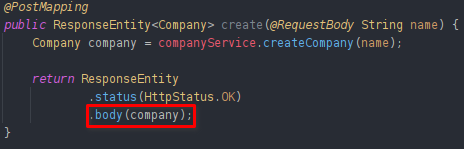
\includegraphics[scale=1.0]{spring_create_method_response.png}
				\caption{\label{fig:spring-create-company} Spring - tworzenie firmy}
			\end{center}
		\end{figure}
	
		\subsubsection{Ruby on Rails}
		W zależności od parametru format framework zwraca zasób w formacie json lub renderuje widok HTML z zasobem.
		\begin{figure}[H]
			\begin{center}
				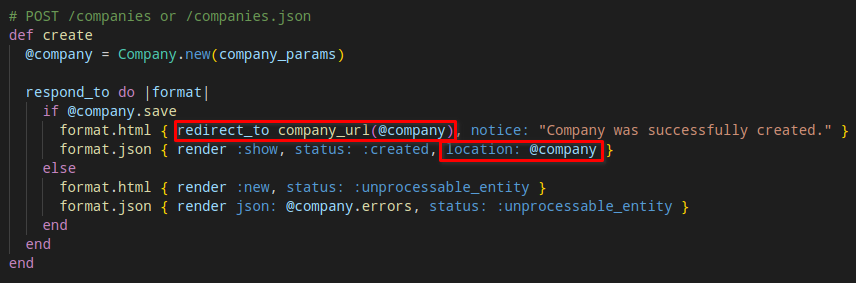
\includegraphics[scale=0.6]{ror_response.png}
				\caption{\label{fig:ror-create-company} Ruby on Rails - tworzenie firmy}
			\end{center}
		\end{figure}
	
	\subsection{JSON czy XML?}
		Współcześnie, uważa się, że XML nie jest najlepszym formatem danych w przypadku REST API. Jest zbyt szczegółowy, trudny do analizy i odczytu. Zdecydowana większość współczesnych API jest oparta o typ JSON. Format ten pożycza niektóre z dobrych stron JavaScriptu i korzysta z bezproblemowej integracji z natywnym środowiskiem przeglądarki \cite{RESTAPIDesignRulebook}. Jeśli nie istnieje jeszcze standardowy format dla danego typu zasobu (np. image/jpeg dla obrazów skompresowanych w JPEG), interfejs REST API powinien używać formatu JSON do strukturyzacji swoich informacji.
	
	\subsection{Błędy}
		Kiedy zajdzie taka potrzeba, API powinno dostarczać użytkownikowi użyteczny komunikat o błędzie w znanym formacie. Odpowiedź z błędem nie powinna różnić się strukturą od standardowych odpowiedzi (np. z aktualizowanym zasobem) \cite{BestPracticesWeb}. API w każdej odpowiedzi powinno zwracać kod statusu HTTP, aby poinformować konsumenta o stanie, w jakim znalazło się zapytania. \\
		Ciało błędów JSON powinno dostarczyć deweloperom:
		\begin{itemize}
			\item przydatny komunikat o błędzie
			\item kod błędu (który jest dokładnie opisany w dokumentacji)
			\item być może szczegółowy opis
		\end{itemize}
		\begin{figure}[H]
			\begin{center}
				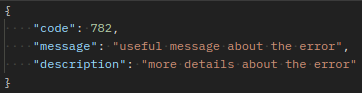
\includegraphics[scale=1.2]{error_example.png}
				\caption{\label{fig:error-message} Odpowiedź z wiadomością o błędzie}
			\end{center}
		\end{figure}
	
		Błędy walidacji dla zapytań POST, PATCH i PUT wymagają dodatkowej informacji o polach zasobu. Dobrym sposobem na poradzenie sobie z tym problemem jest użycie kodu błędu najwyższego poziomu dla błędów walidacji i dostarczenie szczegółowych błędów dla poszczególnych pól:
		\begin{figure}[H]
			\begin{center}
				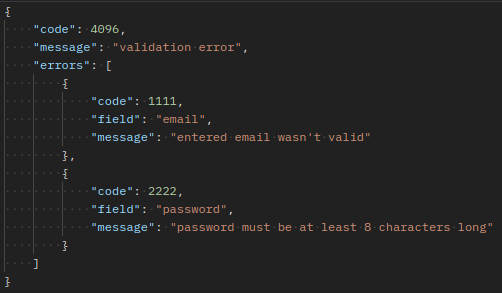
\includegraphics[scale=1.2]{error_validation_example.png}
				\caption{\label{fig:error-validation-message} Odpowiedź z wiadomością o błędzie z opisem pól}
			\end{center}
		\end{figure}
	
		\subsubsection{Ruby on Rails}
		Wygenerowany kod przy pomocy komendy
		\begin{verbatim}
			rails generate scaffold 
		\end{verbatim} 
		służący do stworzenia nowej firmy obsługuje podstawowe błędy. Metoda zwraca odpowiednią wiadomość o błędzie w zależności od przekazanego w zapytaniu parametru określającego typ danych (html/json).

		\begin{figure}[H]
			\begin{center}
				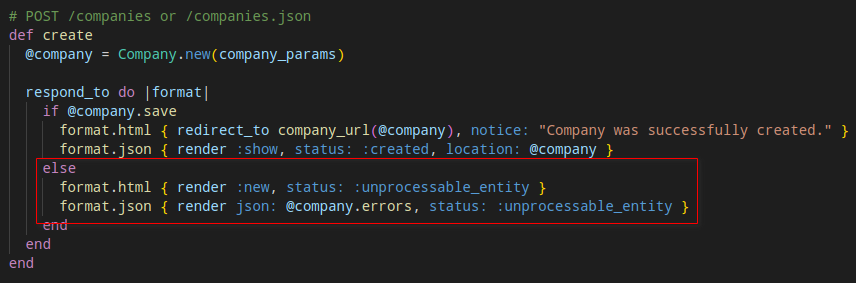
\includegraphics[scale=0.7]{ror_error_handling_ann.png}
				\caption{\label{fig:ror-create-company-error} Ruby on Rails - obsługa błędów}
			\end{center}
		\end{figure}
	
		Dla zapytania, w którym nazwa firmy jest już zajęta np.
		\begin{verbatim}
			http://localhost:3000/companies/?format=json 
			z response body {"company": {"name": "name in use"}}
		\end{verbatim}
		Aplikacja zwróci kod błędu 422 (Unprocessable Entity) wraz z informacją:
		\begin{figure}[H]
			\begin{center}
				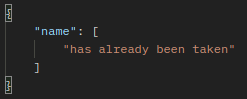
\includegraphics[scale=1.2]{ror_error_name_taken.png}
				\caption{\label{fig:ror-error-name} Ruby on Rails - odpowiedź z wiadomością o błędzie }
			\end{center}
		\end{figure}

		
		\subsubsection{Spring}
		W przypadku Springa nie można liczyć na automatycznie wygenerowany kod. Jednym ze sposobów na poradzenie sobie z obsługą błędów jest, tak jak w przypadku metody stworzonej przy pomocy komendy w Ruby on Rails obsługiwać błędy pojedynczo, ale popularnym rozwiązaniem jest zastosowanie klasy, która przechwytuje wyjątki (na poziomie kontrolera lub globalnie), a następnie zwraca odpowiednią wiadomość dla klienta \cite{SpringDocs}.
		Obsłużenie pojedynczego wyjątku może wyglądać w następujący sposób:
		\begin{figure}[H]
			\begin{center}
				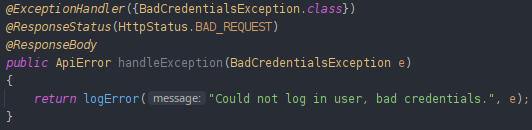
\includegraphics[scale=1.1]{spring_error_handling.png}
				\caption{\label{fig:spring-error-handling} Spring - obsługa wyjątku}
			\end{center}
		\end{figure}
	
		\noindent Z kolei odpowiedź wysłana do aplikacji klienckiej z wiadomością o błędzie może wyglądać w następujący sposób:
		\begin{figure}[H]
			\begin{center}
				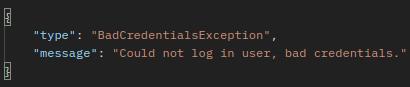
\includegraphics[scale=1.2]{spring_error_postman.png}
				\caption{\label{fig:spring-error-response} Spring - odpowiedź z wiadomością o błędzie}
			\end{center}
		\end{figure}
	
	\subsection{Testowanie}
	Warstwa API każdej aplikacji jest jednym z najbardziej kluczowych komponentów oprogramowania. Jest to kanał, który łączy klienta z serwerem (lub serwis z innym serwisem), napędza procesy biznesowe i zapewnia usługi, które dają namacalną wartość użytkownikom.
	
	Publiczny interfejs API skierowany do klienta, który jest wystawiony na działanie użytkowników końcowych, staje się produktem samym w sobie. Popsucie się go zagraża nie tylko pojedynczej aplikacji, ale całemu łańcuchowi procesów biznesowych zbudowanych wokół niej.
	
	Testy API są szybkie, upraszczają walidację logiki biznesowej, bezpieczeństwa, zgodności i innych aspektów aplikacji. W przypadku, gdy API jest publiczne i zapewnia użytkownikom końcowym programowy dostęp do aplikacji lub usług, testy API efektywnie stają się testami end-to-end i powinny obejmować pełen scenariusz użytkowania funkcjonalności.
	
	\subsubsection{Plan testowania}
	Znaczenie testów API jest oczywiste, ale co i jak powinno się testować w przypadku API? Proces testowania należy rozpocząć od testów funkcjonalnych, aby zapewnić, że interfejs działa poprawnie. Głównymi celami takiego testowania jest:
	\begin{itemize}
		\item zapewnienie, że implementacja działa poprawnie - bez błędów.
		\item zapewnienie, że implementacja działa zgodnie ze specyfikacją wymagań.
	\end{itemize}
	
	Każdy test powinien składać się z kilku punktów, które ten musi spełnić, aby zakończył się powodzeniem:
	\begin{enumerate}
		\item zweryfikowanie poprawności kodu odpowiedzi HTTP. Na przykład, niedozwolone żądanie powinno zwrócić kod 403 (Forbidden).
		\item zweryfikowanie ciała odpowiedzi, poprawności nazw pól, typów i wartości - również w odpowiedziach o błędach.
		\item zweryfikowanie nagłówków odpowiedzi, mają one wpływ zarówno na bezpieczeństwo, jak i wydajność.
		\item opcjonalnie, można sprawdzić poprawność stanu aplikacji, jeśli testy są wykonywane manualnie lub dostęp do UI jest prosty.
		\item zweryfikowanie podstawowej wydajności, jeśli operacja zakończyła się pomyślnie, ale zajęła nieuzasadnioną ilość czasu, test powinien zakończyć się niepowodzeniem.
	\end{enumerate}

	\subsubsection{Kategorie scenariuszy testowych}
	Testy można podzielić na następujące, ogólne grupy scenariuszy testowych:
	\begin{enumerate}
		\item podstawowe testy pozytywne (sprawdzają podstawową funkcjonalność i kryteria akceptacji API).
		\item rozszerzone testy pozytywne z opcjonalnymi parametrami (sprawdzają opcjonalne parametry i dodatkową funkcjonalność).
		\item negatywne testy z ważnymi danymi wejściowymi (sprawdzają, czy aplikacja obsłuży scenariusze problemowe z ważnymi danymi np. rejestracja użytkownika z e-mailem, który nie jest unikalny).
		\item negatywne testy z mniej ważnymi danymi wejściowymi (sprawdzają, czy aplikacja obsłuży scenariusze problemowe z mniej ważnymi danymi np. zmiana wieku użytkownika na wartość tekstową).
		\item testy destrukcyjne (testy, które polegają na celowym zepsuciu API w celu sprawdzenia jego stabilności).
		\item testy bezpieczeństwa, autoryzacji i uprawnień.
	\end{enumerate}
	

\section{Uwierzytelnianie i autoryzacja}
	Podczas obsługi niektórych żądań aplikacja musi wiedzieć, który użytkownik jest za nie odpowiedzialny. Uwierzytelnianie to problem powiązania żądania z użytkownikiem. Z kolei autoryzacja to problem określenia, czy użytkownik ma prawo wykonać daną akcję. Jeśli klient A chce usunąć swoje konto, trzeba mieć absolutną pewność, że to właśnie klient A jest odpowiedzialny za wywołanie akcji (jeśli ustalimy, że tylko właściciel konta może nim zarządzać).
	
	Kiedy klient API wysyła żądanie HTTP, może zawrzeć pewne dane uwierzytelniające w nagłówku HTTP Authorization. Usługa sprawdza poświadczenie i decyduje, czy poprawnie identyfikują one klienta jako konkretnego użytkownika (uwierzytelnianie), oraz czy ten użytkownik jest rzeczywiście upoważniony do zrobienia tego, o co prosi (autoryzacja). Jeśli oba warunki są spełnione, serwer realizuje żądanie \cite{RESTfulWebServices}. Jeżeli brakuje danych uwierzytelniających bądź są one niepoprawne, aby poprawnie obsłużyć żądanie, serwer wysyła komunikat z kodem 401 (Unauthorized). W przypadku kiedy klient uwierzytelnił się poprawnie, ale nie ma prawa na wykonanie akcji, serwer zwraca komunikat 403 (Forbidden).
	
	\subsection{Uwierzytelnianie}
		 
		Najpopularniejszymi sposobami na implementację uwierzytelniania są:
		\begin{itemize}
			\item{Ciasteczka sesyjne} \\
			Po pomyślnym zalogowaniu się użytkownika:
			\begin{enumerate}
				\item serwer generuje token, który jednoznacznie identyfikuje sesję użytkownika.
				\item serwer podpisuje token sekretnym kluczem.
				\item serwer wiąże token z użytkownikiem i zapisuje go w bazie.
				\item serwer wysyła ciasteczko z token do przeglądarki klienta.
				\item przeglądarka otrzymuje ciasteczko i zapisuje je lokalnie.
				\item następnie przeglądarka dołącza ciasteczko do każdego zapytania wysyłanego na serwer.
				\item dla każdego żądania serwer pobiera token z ciasteczka i porównuje go z tym, które zostało zapisane w bazie i jeśli tokeny są takie same, obsługuje żądanie.
			\end{enumerate}
			
			W podejściu opartym na ciasteczkach sesyjnych token nie zawiera żadnych informacji na temat użytkownika, jest jedynie łańcuchem losowych znaków wygenerowanych i podpisanych przez tajny klucz. Token jest zapisywany w bazie danych po stronie serwera w relacji One-to-One z użytkownikiem w celu późniejszej identyfikacji go na podstawie danych w tokenie.
		
			\item{JSON Web Token (JWT)} \\
			Po pomyślnym zalogowaniu się użytkownika:
			\begin{enumerate}
				\item serwer generuje JWT token i szyfruje go.
				\item serwer wysyła token do przeglądarki klienta.
				\item przeglądarka otrzymuje token i zapisuje go lokalnie.
				\item następnie przeglądarka dołącza token do każdego zapytania wysyłanego na serwer przy pomocy nagłówka Authorization.
				\item dla każdego żądania serwer pobiera token z nagłówka Authorization, odszyfrowuje go i wydobywa dane o użytkowniku i jego uprawnieniach. Opierając się wyłącznie na danych z tokena, jest w stanie zaakceptować lub odrzucić żądanie klienta.
			\end{enumerate}
		
			W podejściu JWT sam token jest w stanie jednoznacznie zidentyfikować użytkownika, więc token nie jest przechowywany w żadnej bazie danych po stronie serwera. Wszystkie potrzebne informacje o użytkowniku są przechowywane w tokenie JWT.
			
			\subsubsection{OAuth}
			OAuth jest otwartym protokołem, który pozwala użytkownikom zweryfikować się za pomocą zaufanego podmiotu trzeciego (Google, Microsoft Azure czy Facebook) poprzez wymianę tokenów, aby uzyskać dostęp do aplikacji. Najnowsza wersja protokołu, OAuth 2.0 jest uważana za standard w branży i wykorzystywana przez największe firmy.
			
			Największą zaletą korzystania z OAuth jest przerzucenie odpowiedzialności za zarządzanie hasłami na podmioty zewnętrzne. Zmniejsza to ilość przechowywanych danych użytkowników oraz przyśpiesza proces tworzenia aplikacji. Co więcej, użytkownicy nie potrzebują nowego konta i hasła w celu korzystania z usługi, ponieważ posługują się już istniejącym kontem. 
		\end{itemize}
	
	\subsection{Autoryzacja}
		Celem autoryzacji jest sprawdzenie, czy użytkownik jest uprawniony do korzystania z określonego zasobu (np. tylko administrator może wyświetlić stronę z listą wszystkich użytkowników serwisu). Autoryzację najczęściej implementuje się za pomocą ról. Oznacza to, że każdemu użytkownikowi jest przypisana rola (np. ADMIN, EMPLOYEE, CLIENT), którą przechowuje się w bazie danych. Następnie, dla każdego żądania, które wymaga konkretnych uprawnień, serwer sprawdza, czy klient jest upoważniony do wykonania akcji.

\section{Plan tworzenia serwisu Restful \cite{RESTfulWebServices}}
	Przed rozpoczęciem programowania REST API warto stworzyć plan, który ułatwi i ustandaryzuje proces tworzenia oprogramowania. Poniższa procedura zawiera wszystkie standardowe kroki, które należy zrealizować, aby dodać nową funkcjonalność do REST API. Trzymanie się takiego planu ułatwi deweloperom pracę z API oraz pozwoli uniknąć wielu błędów.
	
\begin{enumerate}
	\item Ustal zestaw danych.
	\item Podziel zestaw danych na zasoby. \\~\\
	Dla każdego zasobu:
	\item Nazwij zasób przy pomocy URI.
	\item Udostępnij endpointy potrzebne do korzystania z zasobu.
	\item Zaprojektuj reprezentacje zasobu przesyłaną do serwera przez klienta.
	\item Zaprojektuj reprezentacje zasobu udostępnianą dla klienta.
	\item Zintegruj nowy zasób z istniejącymi zasobami.
	\item Rozważ typowe flow związane z zasobem (co powinno się z nim stać?).
	\item Rozważ, w jakich sytuacjach mogą wystąpić błędy (co może pójść nie tak?).
\end{enumerate}


%\chapter{Praktyczne problemy (opis specyficznych problemów wraz z możliwymi rozwiązaniami, case by case)}

\section{frameworki}
\subsection{Spring, Jsbs}
\subsection{Ruby on Rails, Ruby}
\subsection{porównanie frameworków}
\subsection{dlaczego te frameworki? po co 2?}

\section{Standardowe (CRUD)}
\section{Nested}
\section{Filtrowanie, sortowanie, wyszukiwanie}
\section{inne}

\addcontentsline{toc}{chapter}{Zakończenie}
\chapter*{Zakończenie}
Praca przedstawiła podstawowe koncepty związane z tworzeniem REST API. Na początku pokazany i opisany został protokół HTTP oraz jego rozszerzenie - HTTPS. W pracy zawarte zostały podstawowe informacje na temat metod HTTP oraz popularnych kodów odpowiedzi, które należy wykorzystywać w architekturze REST. W kolejnej części praca skupiła się na istocie REST API, a więc samej architekturze REST oraz zasadach, które należy przestrzegać, by określić serwis RESTowym. Rozdział drugi, „Tworzenie REST API” położył nacisk na praktyczne aspekty programowania interfejsu sieciowego. Rozpoczął się od sekcji dobrych praktyk, gdzie opisany został szereg istotnych elementów przy tworzeniu REST API, od dokumentacji i wersjonowania oprogramowania po obsługę błędów oraz testowanie. Następnie praca przedstawiła dwa mechanizmy, które pozwalają na implementację uwierzytelniania użytkowników, opisała, czym jest OAuth oraz wytłumaczyła na czym polega autoryzacja. W ostatniej sekcji zademonstrowany został plan, który warto znać podczas projektowania REST API.

W dobie ciągłego przepływu informacji w sieci Internet należy tworzyć REST API, które są przyjemne w użytkowaniu oraz zdatne do utrzymania w celu zmaksymalizowania swojej atrakcyjności dla potencjalnych klientów. Współcześnie, wykrystalizowały się pewnie branżowe standardy, których warto trzymać się przy implementacji REST API.

W tej pracy wytłumaczono, czym właściwie jest REST API oraz przedstawiono wiele praktyk, które warto wdrożyć podczas programowania interfejsów sieciowych, aby dostarczyć użytkownikom oprogramowania produkt wysokiej jakości..

%now enable appendix numbering format and include any appendices
\appendix
\addcontentsline{toc}{chapter}{Spis tabel i rysunków}
\chapter*{Spis tabel i rysunków}
\begingroup
\let\clearpage\relax

\listoftables
\listoffigures

\endgroup

%\chapter*{Załączniki}

%next line adds the Bibliography to the contents page
\addcontentsline{toc}{chapter}{Bibliografia}
%uncomment next line to change bibliography name to references
%\renewcommand{\bibname}{References}
\bibliography{refs}        %use a bibtex bibliography file refs.bib
\bibliographystyle{plain}  %use the plain bibliography style

\end{document}

